\setcounter{chapter}{5}
\chapter{Onde elettromagnetiche}

\section{Equazioni di Maxwell nel vuoto}

Il campo elettrico $\bold{E}(\bold{r},t) $ e il campo magnetico $\bold{B}(\bold{r},t)$ esistono quando sono presenti condizioni non stazionarie per la densit\`a di carica libera  $\rho(\bold{r},t)$ e la densit\`a di corrente libera $\bold{J}(\bold{r},t)$. L'interazione tra le cariche \`e descritta dalla forza $\bold{F} = q(\bold{E} + \bold{v} \times \bold{B})$ e le equazioni di Maxwell nel vuoto descrivono la relazione tra i campi  e le sorgenti:
\begin{align}
	& \nabla \cdot \bold{E} = \frac{\rho}{\varepsilon_0} \quad \text{Legge di Gauss} \\ \rule{0pt}{20pt}
	&\nabla \times \bold{E} = - \frac{\partial \bold{B}}{\partial t} \quad \text{Legge di Faraday} \\ \rule{0pt}{20pt}
	& \nabla \cdot \bold{B} = 0 \\ \rule{0pt}{20pt}
	& \nabla \times \bold{B} = \mu_0 \bold{J} + \varepsilon_0 \mu_0 \frac{\partial \bold{E}}{\partial t} \quad \text{Legge di Amp\`ere-Maxxwell}
\end{align}
Nel limite statico le soluzioni per $\bold{E}$ e $\bold{B}$ sono indipendenti, infatti le equazioni di Maxxwell assumono la forma 
\begin{equation*}
\left \{ \begin{array}{l}
	 \nabla \cdot \bold{E} = \frac{\rho}{\varepsilon_0}  \quad \quad  \nabla \cdot \bold{B} = 0 \\ \rule{0pt}{20pt}
	 \nabla \times \bold{E} = 0 \quad \quad  \nabla \times \bold{B} = \mu_0 \bold{J}\\ 
	\end{array}\right.
\end{equation*}
Nel limite quasi statico, il campo elettrico variabile dipende da $\bold{B}$, ma non il viceversa. Le soluzioni risultano dunque essere pi\`u complesse rispetto al caso statico perch\`e si hanno campo elettrico e campo magnetico accoppiati dalla legge di Faraday e dalla leggi di Ampere-Maxxwell.

Dallo studio di alcune configurazioni idealizzante, la cui relazioni tra campi e sorgenti \`e di facile deduzione, emergono delle propriet\`a principali della soluzione delle equazioni di Maxwell: 
\begin{itemize}
	\item \textit{principio di casualit\`a }: sorgenti variabili generano una perturbazione del campo magnetico che si propaga nel vuoto con velocit\`a $c$ pari a quella della luce. Poich\`e l'informazione si propaga con una velocit\`a finita $c$, il campo osservabile ad una certa distanza dalla sorgente \`e un campo che riflette ci\`o che \`e avvenuto alla sorgente ad un tempo precedente.
	\begin{equation*}
		\bold{E}(\bold{r},t) = \bold{E}\left(t - \frac{|r|}{c}\right) \quad \quad \bold{B}(\bold{r},t) = \bold{B} \left(t - \frac{|r|}{c}\right)
	\end{equation*}
	\item per le leggi sul flusso di $\bold{E}$ e $\bold{B}$, la perturbazione del campo \`e ortogonale alla direzione di propagazione. 
	\item per le leggi di Faraday e Amp\`ere-Maxxwell, il campo elettrico e magnetico variabili si autosostengono, sono mutualmente ortogonali, e hanno ampiezza legate dalla relazione 
	\begin{equation*}
		B = \frac{1}{c}E
	\end{equation*}
	\item la velocit\`a di propagazione della perturbazione \`e  
	\begin{equation*}
		c = \frac{1}{\sqrt{\varepsilon_0 \mu_0}}
	\end{equation*}
\end{itemize}

\subsection{Soluzioni ondulatorie delle equazioni di Maxxwell nel vuoto e all'esterno delle sorgenti}

La derivazione formale della propagazione per onde dei campi elettromagnetici nel vuoto la si ottiene scrivendo le equazioni di Maxxwell in regioni prive di sorgenti, $\rho(\bold{r},t) = 0$ e $\bold{J}(\bold{r},t) = 0$
\begin{equation*}
\left \{ \begin{array}{l}
	 \nabla \cdot \bold{E} = 0  \quad \quad \quad \quad   \nabla \cdot \bold{B} = 0 \\ \rule{0pt}{20pt}
	 \nabla \times \bold{E} = - \frac{\partial \bold{B}}{\partial t} \quad \quad  \nabla \times \bold{B} = \varepsilon_0 \mu_0 \frac{\partial \bold{E}}{\partial t}\\ 
	\end{array}\right.
\end{equation*}
Per disaccoppiare le equazioni applichiamo l'operazione di rotore ad entrambi i membri della legge di Faraday e di Amp\`ere-Maxxwell, e utilizziamo l'identit\`a vettoriale 
\begin{equation*}
	\nabla \times (\nabla \times \bold{A} ) = - \nabla ^2\bold{A} + \nabla (\nabla \cdot \bold{A})
\end{equation*}

Sostituendo $\bold{A} = \bold{E}$ si ha che 
\begin{equation*}
	\nabla \times (\nabla \times \bold{E}) = - \nabla^2 \bold{E} + \nabla (\underbrace{\nabla \cdot \bold{E}}_{=0}) = - \frac{\partial }{\partial t}(\nabla \times \bold{B})
\end{equation*}
restandoci l'equazione
\begin{equation}
	\nabla^2 \bold{E} = \varepsilon_0 \mu_o\frac{\partial^2 \bold{E}}{\partial t^2}
\end{equation}
analogamente ponendo $\bold{A} = \bold{B}$ si ha l'equazione:
\begin{equation}
	\nabla^2 \bold{B} = \varepsilon_0 \mu_0 \frac{\partial^2 \bold{B}}{\partial t^2}
\end{equation}
che hanno la stessa struttura dell'equazione delle onde di D'Alambert:
\begin{equation*}
	\nabla^2f = \frac{1}{c^2} \frac{\partial ^2f}{\partial t^2}
\end{equation*}
Le equazioni di Maxxwell in vuoto e in regioni prive di sorgenti hanno soluzioni ondulatorie. Confrontando le equazioni (6.6) e (6.5) con l'equazione di D'Alambert scopiamo che le onde elettromagnetiche nel vuoto si propagano alla velocit\`a 
\begin{equation*}
	c = \frac{1}{\sqrt{\varepsilon_0 \mu_0}}
\end{equation*}
Le misure sperimentali della velocit\`a della luce e di $1/\sqrt{\varepsilon_0 \mu_0}$ ci dicono che la luce \`e radiazione elettromagnetica.
\begin{remark}
\
\begin{itemize}
	\item Le equazioni (6.5) e (6.6)  ammettono soluzioni anche per campi che non soddisfano le equazioni di Maxxwell, tali soluzioni non possono descrivere campi elettromagnetici reali.
	\item Le equazioni (6.5) e (6.6) sono soddisfatte anche da campi uniformi e costanti, tali campi non hanno le caratteristiche di un'onda.
\end{itemize}	
\end{remark}
\section{Tipi di onda soluzione dell'equazione di D'Alambert}
\subsection{Onde piane}
\begin{wrapfigure}{r}{0.5\textwidth}  % 'r' for right, 'l' for left
  \centering
  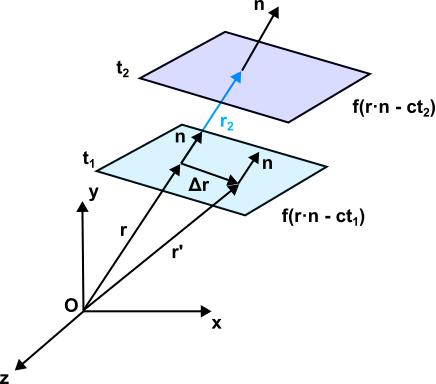
\includegraphics[width=0.49\textwidth]{images/planar_wave}
\end{wrapfigure}
Una delle soluzioni dell'equazione di D'Alambert tridimensionale \`e data da un'onda piana scalare, ed \`e rappresentata da una funzione
\begin{equation}
	f = f(\bold{r} \cdot \hat{n} \;\mp \; ct)
\end{equation}
dove il vettore
\begin{equation*}
	\bold{r} = x \hat{u}_{x} + y \hat{u}_{y} + z \hat{u}_{z}
\end{equation*}
\`e il raggio vettore che individua un punto nello spazio in un riferimento cartesiano, $\hat{n}$ \`e il versore che individua la direzione di propagazione dell'onda e $c$ \`e la velocit\`a con cui questa si propaga. Il prodotto vettoriale $\bold{r} \cdot \hat{n}$ \`e la proiezione della posizione del punto lungo la direzione di propagazione dell'onda.

La funzione f \`e definita in tutto lo spazio-tempo ed assume lo stesso valore (fronte d'onda) in tutti i punti in ci il suo argomento $\xi = \bold{r} \cdot \hat{n}  \; \mp \; ct$ (detta fase), ha lo stesso valore. Per ogni istante fissato, il luogo dei punti in cui f ha  un determinazione valore \`e un piano ortogonale alla direzione di propagazione dell'onda. Per dimostrarlo, osserviamo che 
\begin{equation*}
	f(\xi) = f(\xi') \quad \iff \quad \xi = \xi'
\end{equation*}
ad un istante $t$ fissato. Questo vuol dire che 
\begin{equation*}
	\bold{r} \cdot \hat{n} \pm ct = \bold{r}' \cdot \hat{n} \pm ct \quad \iff \quad (\bold{r}-\bold{r}') \cdot \hat{n} = 0 
\end{equation*}
questo vuol dire che $\Delta \bold{r}$ \`e appartiene ad un piano ortogonale alla direzione $\hat{n}$. 

Il fatto che l'onda piana si propaghi con una velocit\`a c lo si dimostra dal fatto che 
\begin{equation*}
	f(\xi_{1}) = f(\xi_{2}) \quad \iff \quad \xi_{1} = \xi_{2} 
\end{equation*}
questo equivale a chiedere che 
\begin{equation*}
	\bold{r}_{1} \cdot \hat{n} \pm ct_{1} = \bold{r}_{2} \cdot \hat{n} \pm ct_{2} \quad \iff \quad \Delta \bold{r} \cdot \hat{n} = \pm c(t_{2}-t_{1}) \quad \iff \quad \frac{\Delta \bold{r}}{\Delta t} \cdot \hat{n} =  \pm c
\end{equation*}
dimostrando che i piani in cui f \`e costante si propagano lungo la direzione $\hat{n}$ con velocit\`a $\pm c $ per onde progressive e regressive. In alternativa si pu\`o calcolare la veloicit\`a con cui si propaga il fronte d'onda d'onda imponendo: 
\begin{equation*}
	\frac{d \xi }{dt} = 0 \quad \Rightarrow \quad \frac{d \bold{r}}{dt} = \pm c
\end{equation*}
e prede il nome di \textbf{velocit\`a di fase}.

A questo punto non ci resta da dimostra per sostituzione come l'equazione (6.7) sia soluzione dell'equazione di D'Alambert tridimensionale:
\begin{equation*}
	\nabla^2 f(\bold{r} \cdot \hat{n} \mp ct) =\frac{1}{c^2}\frac{\partial^2 f(\bold{r} \cdot \hat{n} \mp ct)}{\partial t^2} 
\end{equation*}
mostrando come il termine di sinistra sia uguale a quello di destra e viceversa.

In generale in coordinate cartesiane abbiamo che per ciascuna componente:
\begin{equation*}
	\frac{\partial f}{\partial x} = \frac{\partial f}{\partial \xi} \frac{\partial \xi}{\partial x}
\end{equation*}
siccome $\xi = xn_{x} + yn_{y} + zn_{z} \mp ct $ si ha che ciascuna derivata \`e della forma:
\begin{equation*}
	\left \{ \begin{array}{l}
		\frac{\partial f}{\partial x} = n_{x} \frac{\partial f}{\partial \xi} \\ \rule{0pt}{20pt}
		\frac{\partial f}{\partial y} = n_{y} \frac{\partial f}{\partial \xi} \\ \rule{0pt}{20pt}
		\frac{\partial f}{\partial z} = n_{z} \frac{\partial f}{\partial \xi}
	\end{array}\right.
\end{equation*}
possiamo esprimere dunque l'operatore
\begin{equation*}
	\nabla = (n_{x} \hat{u}_{x} + n_{y} \hat{u}_{y} + n_{z} \hat{u}_{z}) \frac{\partial }{\partial \xi} = \hat{n} \frac{\partial }{\partial \xi} 
\end{equation*}
e quindi
\begin{equation*}
	\nabla^2 = \nabla \cdot \nabla = \hat{n} \frac{\partial }{\partial \xi} \cdot \hat{n} \frac{\partial }{\partial \xi} = \frac{\partial^2}{\partial \xi^2}
\end{equation*}
analogamente la derivata temporale pu\`o essere scritta come
\begin{equation*}
	\frac{\partial f}{\partial t} = \frac{\partial f }{\partial \xi} \frac{\partial \xi}{\partial t} = \mp c \frac{\partial f}{\partial \xi}
\end{equation*}
se deriviamo rispetto al tempo una seconda volta otteniamo
\begin{equation*}
	\frac{\partial^2 f }{\partial t^2} = c^2 \frac{\partial ^2f}{\partial \xi ^2}
\end{equation*}
e quindi i termini sia di destra che di sinistra coincidono.

\section{Onde piane monocromatiche}



